\documentclass[titlepage]{article}

\usepackage{./estilos/estiloBase} % Basicamente son todas las
                                  % librerias usadas. En caso de que
                                  % falten librerias se van añadiendo
                                  % al fichero.
\usepackage{./estilos/colores}  % Algunos colores ya generados, para
                                % los algunos estilos más avanzados.
\usepackage{./estilos/comandos} % Algunos comandos personalizados

\author{Manuel de la Calle Brihuega\\Jose Marente Florín\\David Saltares Márquez}
\title{Granny's Bloodbath\\Manual de usuario}

% Portada
% Índice
% Introducción
% Descarga e instalación
% Requisitos mínimos
% Historia y personajes
% Pantallas
% Jugar
% Creación de niveles
% Créditos
% Licencia
% Contacto y soporte

\setlength{\unitlength}{1 cm} %Especificar unidad de trabajo

\begin{document}

% ------- %
% PORTADA %
% ------- %

\thispagestyle{empty}
\begin{picture}(18,4)
\put(-2.1,0){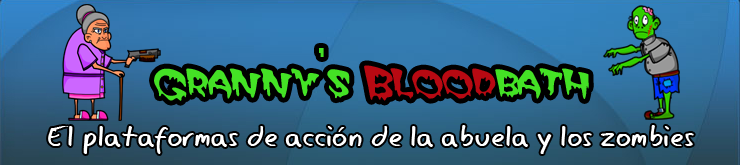
\includegraphics[scale=0.6]{portada.png}}
\end{picture}\\[4cm]

\begin{center}
\textbf{{\Huge Manual de usuario}}\\[1cm]
\textbf{{\large v0.1 BETA}}\\[4cm]
{\large David Saltares Márquez}\\
{\large Jose Marente Florín}\\
{\large Manuel de la Calle Brihuega}\\[2.2cm]
Este documento posee una licencia GPL 3
\end{center}
\clearpage

\tableofcontents
\clearpage

\section{Introducción}
Bienvenido al manual de \emph{Granny's Bloodbath}, si estás leyendo esto es que estás mínimamente interesado en lo que hemos hecho lo que nos honra enormemente. \emph{Granny's Bloodbath} es un juego de plataformas y acción protagonizado por una abuelita. Ha sido desarrollado para la asignatura de Diseño de Videojuegos en la Universidad de Cádiz en C++ utilizando la librería SDL. Te deseamos que lo pases lo mejor posible y que aniquiles a todos los zombies que puedas, ¡salva a la abuelita!\\

A lo largo del manual verás los requisitos mínimos, una brevísima guía de instalación, los detalles de la historia y sus personajes así como los controles básicos. A continuación, la sección más interesante de este manual: \textbf{crear tus propios niveles para el juego}. Sería genial que colaboraras con la comunidad y aportaras tu granito de arena a nuestro trabajo.\\

\emph{Granny's Bloodbath} es Software Libre y se distribuye bajo una licencia GPL. Básicamente puedes distribuirlo con toda libertad así como consultar su código fuente o modificarlo. Para más detalles sobre la licencia GPL puedes consultar el anexo correspondiente.\\

¡Que disfrutes!


\clearpage

\section{Requisitos mínimos}
No es que necesites un maquinón para disfrutar de \emph{Granny's Bloodbath} pero olvídate de matar zombies si tienes un 286 de hace 30 años. Para jugarlo dignamente necesitas al menos:

\begin{itemize}
	\item \emph{Procesador:} Intel, AMD o sucedáneos de al menos 800MHz.
	\item \emph{Memoria RAM:} 64MB.
	\item \emph{Disco duro:} 30MB libres.
	\item \emph{Pantalla:} 960x544px de resolución.
	\item \emph{Sistema operativo:} GNU/Linux o Microsoft Windows
	\item \emph{Entrada:} un teclado de los 20 duros será suficiente.
	\item \emph{Tarjeta de sonido:} con cualquiera nos vale.
\end{itemize}


\clearpage

\section{Descarga e instalación}
Descargar e instalar \emph{Granny's Bloodbath} es de lo más sencillo, a continuación explicamos el proceso.

\begin{itemize}
	\item Entra en la sección de descargas del blog oficial:\\
		\href{http://grannysbloodbath.wordpress.com/descargas/}{http://grannysbloodbath.wordpress.com/descargas/}
	\item Elije la última versión disponible acorde con tu sistema operativo y descárgala
	\item Según tu sistema deberás realizar uno de los siguientes pasos:
\end{itemize}

\subsection{Instalación en Windows}
Descomprime el fichero obtenido en el directorio deseado y... ¡Listo, ya puedes jugar!\\

Puede que en un futuro creemos un setup que permita elegir directorio de instalación así como creación de accesos directos. No obstante, por el momento creemos que así es suficiente. Cuanto más sencillo mejor, ¿no?

\subsection{Instalación en GNU/Linux}
Descomprime el fichero obtenido en el directorio deseado.\\

Debes tener instalados los paquetes: libsdl, libsdl-mixer, libsdl-image, libsdl-ttf. Si no los tienes abre una terminal y escribe:

\lstinputlisting[style=consola]{paquetes.sh}

Es probable que no puedas ejecutar el juego por problemas con los permisos, si ese es tu caso debes de hacer lo siguiente en la terminal:

\lstinputlisting[style=consola]{permisos.sh}

Vale, ha sido un proceso un poco más largo pero... ¡Ya puedes jugar! Puede que más adelante creemos un paquete \emph{.deb} para que la instalación sea mucho más sencilla.


\clearpage

\section{Historia y personajes}
\subsection{Historia}
La protagonista es una abuelita octogenaria que vive plácidamente en su casita situada en una agradable zona residencial. Todo iba de maravilla hasta que se ve invadida por terribles zombies. Es entonces cuando, lo que parecía una inocente y respetable abuela (como la que podemos tener todos nosotros), decide arrastrar con ella a todos los engendros que pueda de camino al infierno. ¿Será nuestra abuelita un digno rival para el apocalipsis que se presenta?.\\

¡Ayúdala en su periplo por el apocalipsis!

\subsection{La abuelita}
Debajo de esa bata y ese camisón (no le dio tiempo de cambiarse cuando la atacaron los zombies) se esconde una bestia iracunda. Su descanso se ha visto interrumpido y esos putrefactos zombies maleducados deben pagar por ello.

\begin{center}
	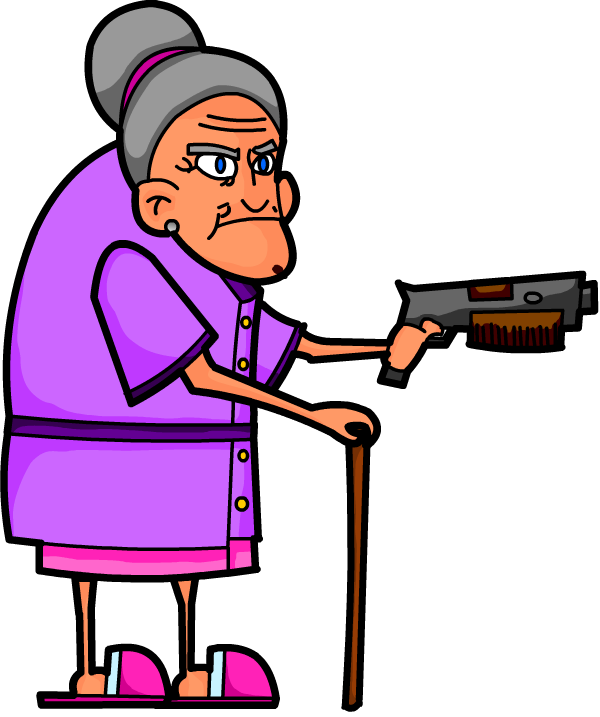
\includegraphics[scale=0.2]{granny.png}
\end{center}

\subsection{La horda}
¡Cuidado con los zombies! Te encontrarás con distintos tipos a lo largo del juego y debes trazar la mejor estrategia posible para enfrentarte a cada uno de ellos ya que tienen habilidades distintas:

\begin{center}
	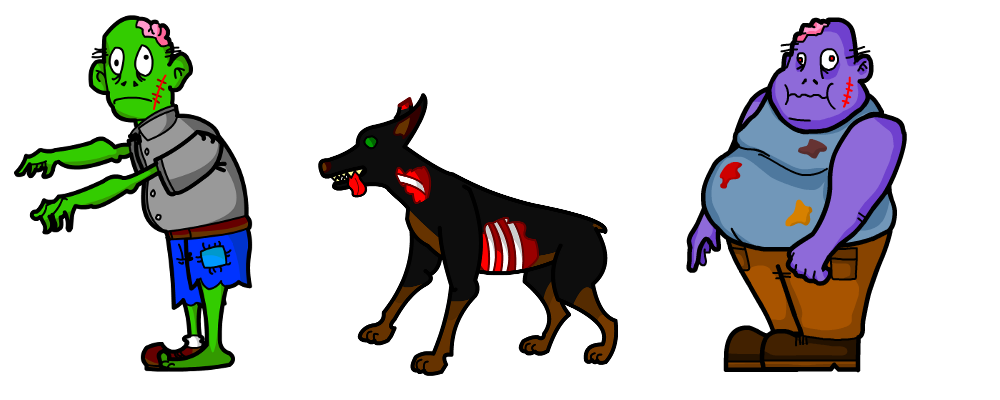
\includegraphics[scale=0.35]{enemigos.png}
\end{center}

\begin{itemize}
	\item \emph{Zombie genérico:} El clásico enemigo que se repite en todos los juegos y nosotros no tenemos la decencia siquiera de cambiarlo de color. Se moverá torpemente persiguiendo a ala abuela y si te toca serñas dañando. Es sencillo de eliminar.
	\item \emph{Perro zombie rabioso:} Con una clara inspiración de la saga Resident Evil (¡Shhhhh que nos pediran derechos de autor!) llega este sabueso asesino. Su velocidad pondrá nervioso a más de uno así que ten cuidado, no podrás huir.
	\item \emph{Zombie gordo:} En otra vida fue cliente honorífico de cierta cadena de hamburgueserías americana y ahora no para de devolver lo que un día zampó. Es cierto que se mueve con extrema lentitud pero sus vómitos corrosivos (aparte que dan un asco tremendo) pueden acabar contigo en un plis plas.
\end{itemize}

\paragraph{}
¡Cuidado! Puede que en la aventura de la abuelita te topes con otros enemigos mucho más terribles que los anteriores.

\subsection{Los preciados items}
¡La abuelita no está sóla! Cuenta con diversos objetos que la ayudarán en su objetivo. ¡Se inteligente, audaz y encuéntralos todos para sobrevivir!

\begin{center}
 	
\includegraphics[scale=0.6]{items.png}
\end{center}

\begin{itemize}
	\item \emph{Dentaduras postizas:} ¿Qué sería de una abuelita sin sus dentaduras postizas? Estarán en las zonas más inaccesibles de cada nivel pero obtendrás puntos al recogerlas y si consigues 10, ganarás una vida.
	\item \emph{Pastillas para la tensión:} Los zombies pueden hacer mella en una abuelita fácilmente así que recogiendo tus queridas pastillas recuperarás parte de tu energía.
	\item \emph{Munición de la escopeta:} Decidida a acabar con todos los zombies, la abuela recoge la escopeta de su difunto marido. ¡No te apresures disparando! La muninción es limitada y la recuperarás recogiendo estos objetos.
\end{itemize}


\clearpage

\section{Jugar}
\subsection{Menu principal}
Cuando inicias \emph{Granny's Bloodbath} comienzas en el menú principal. Con las teclas de dirección puedes moverte por las distintas opciones:

\begin{center}
	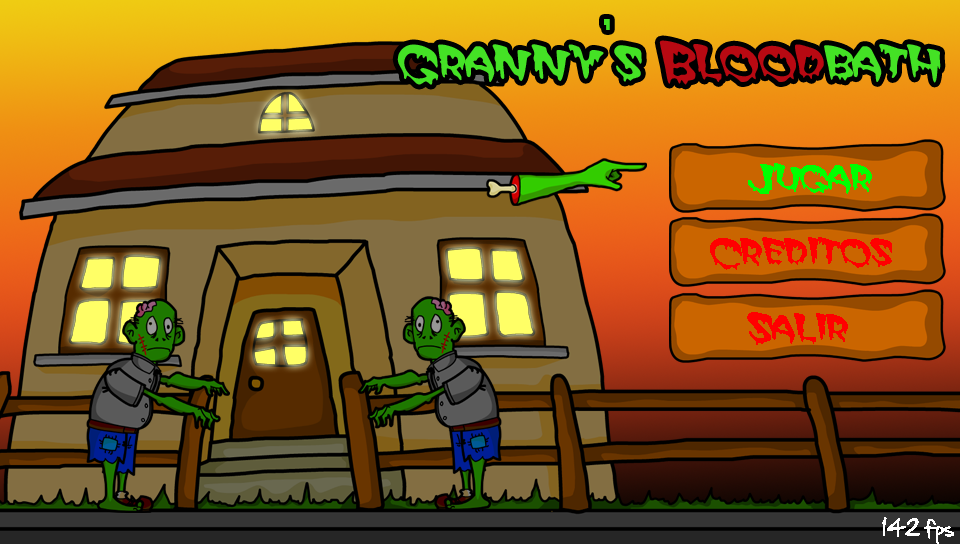
\includegraphics[scale=0.35]{screen-menu.png}
\end{center}

\begin{itemize}
	\item \emph{Jugar:} comienzas una nueva partida o continuas la que habías dejado a medias
	\item \emph{Créditos:} puedes ver las grandes personas que han desarrollado o contribuido a desarrollar \emph{Granny's Bloodbath}
	\item \emph{Salir:} cierras el juego pero no quieres eso, ¿verdad?
\end{itemize}

Para seleccionar una pulsa la barra espaciadora.

\subsection{¡Quiero jugar!}
Bien, has elegido comenzar la aventura. En \emph{Granny's Bloodbath} existen dos tipos de escenas: las de historia y las de juego. 

\begin{itemize}
	\item \emph{Escenas de historia: } se nos cuenta algún fragmento de la aventura de nuestra abuelita. Podemos escuchar al narrador o pulsar \emph{ESCAPE} para avanzar.
	\item \emph{Escenas de juego: } la acción, la sangre y toda la diversión se encuentran concentradas en los niveles del juego. A continuación explicamos el significado de los indicadores que aparecen en pantalla así como los controles para manejar a la abuelita. Si lo que quieres es crear tus propios escenarios debes avanzar un poco más.
\end{itemize}

Cuando comiences a jugar verás una pantalla semejante a esta:

\begin{center}
	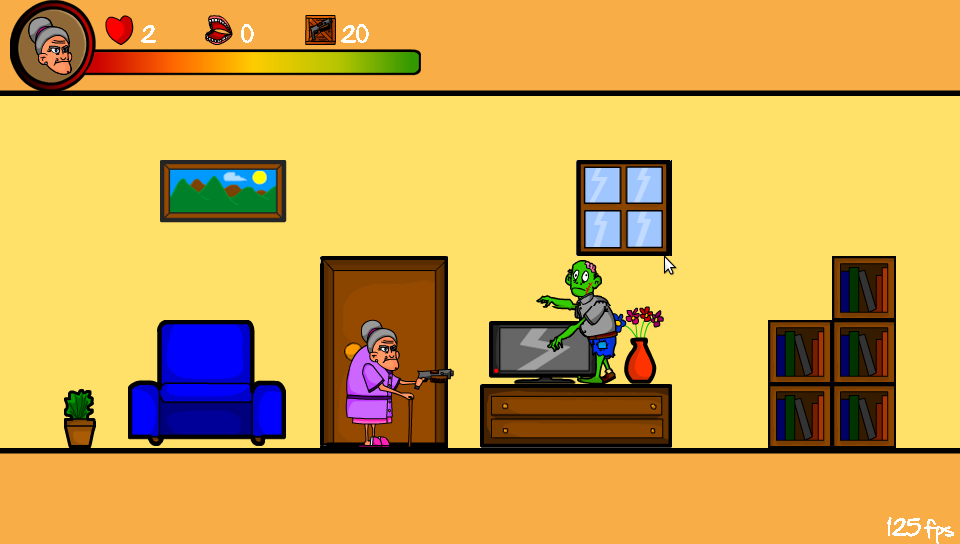
\includegraphics[scale=0.35]{screen-juego.png}
\end{center}

\subsubsection{HUD}
El HUD es la zona donde se encuentran los indicadores que nos informan sobre el estado de la abuelita. Tiene los siguientes componentes:

\begin{center}
	
\includegraphics[scale=0.35]{hud.png}
\end{center}

\begin{itemize}
	\item \emph{Barra de vida}: Disminuye con los ataques zombie, ¡ten cuidado, si llega a 0 perderás una vida!
	\item \emph{Corazones}: Número de vidas disponibles. Si te eliminan y te quedan vidas volverás a empezar el nivel pero si no te quedan tendrás que empezar la aventura desde el principio.
	\item \emph{Dentaduras}: Puntos, si consigues un número determinado se te obsequiará con una vida adicional
	\item \emph{Munición}: La munición de la escopeta es limitada, ten cuidado, no la malgastes y consigue todas las cajas de munición. Disparar a distancia es una gran ventaja.
\end{itemize}

\subsubsection{Controles}
Estamos seguros que el diagrama que viene a continuación solventará todas tus dudas sobre los controles del juego:

\begin{center}
	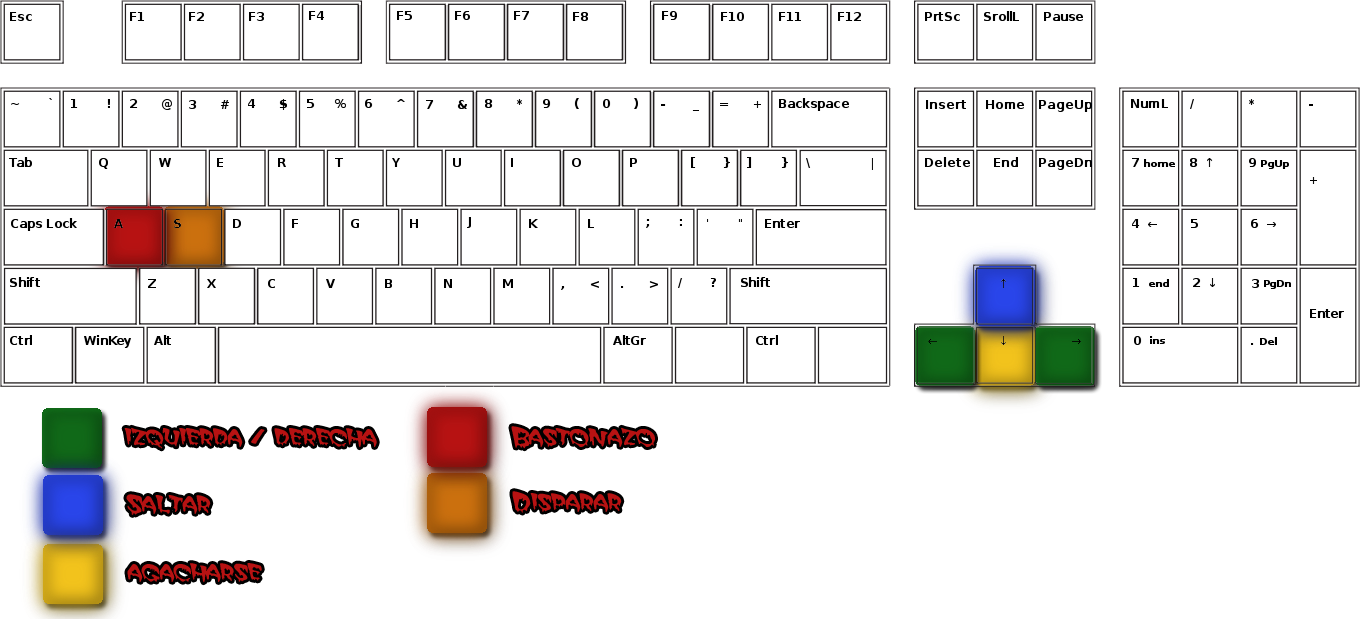
\includegraphics[scale=0.35]{controles.png}
\end{center}


\clearpage

\section{Creación de niveles}
Para editar los niveles te proponemos un sistema bastante sencillo, el
mismo que hemos utilizado nosotros. Se trata de Tiled, una herramienta libre
y multiplataforma escrita en Java aunque también tienen una versión con Qt.
A continuación os proponemos los pasos para descargarla, instalarla y crear
niveles con ella. ¡Anímate, es muy sencillo!

\subsection{Descargando Tiled}
Para poder usar Tiled necesitas el Java Runtime Enviroment (JRE), la máquina
virtual de Java ya que es el entorno que utiliza. Una vez instalado el JRE
sólo tienes que acudir a su web principal:\\

\href{http://mapeditor.org}{http://mapeditor.org}\\

Aunque también podéis descargarlo directamente a través de este enlace:\\

\href{http://sourceforge.net/projects/tiled/files/Tiled/tiled-0.7.2-bin.zip}{http://sourceforge.net/projects/tiled/files/Tiled/tiled-0.7.2-bin.zip}

\subsection{Utilizando Tiled}

\begin{center}
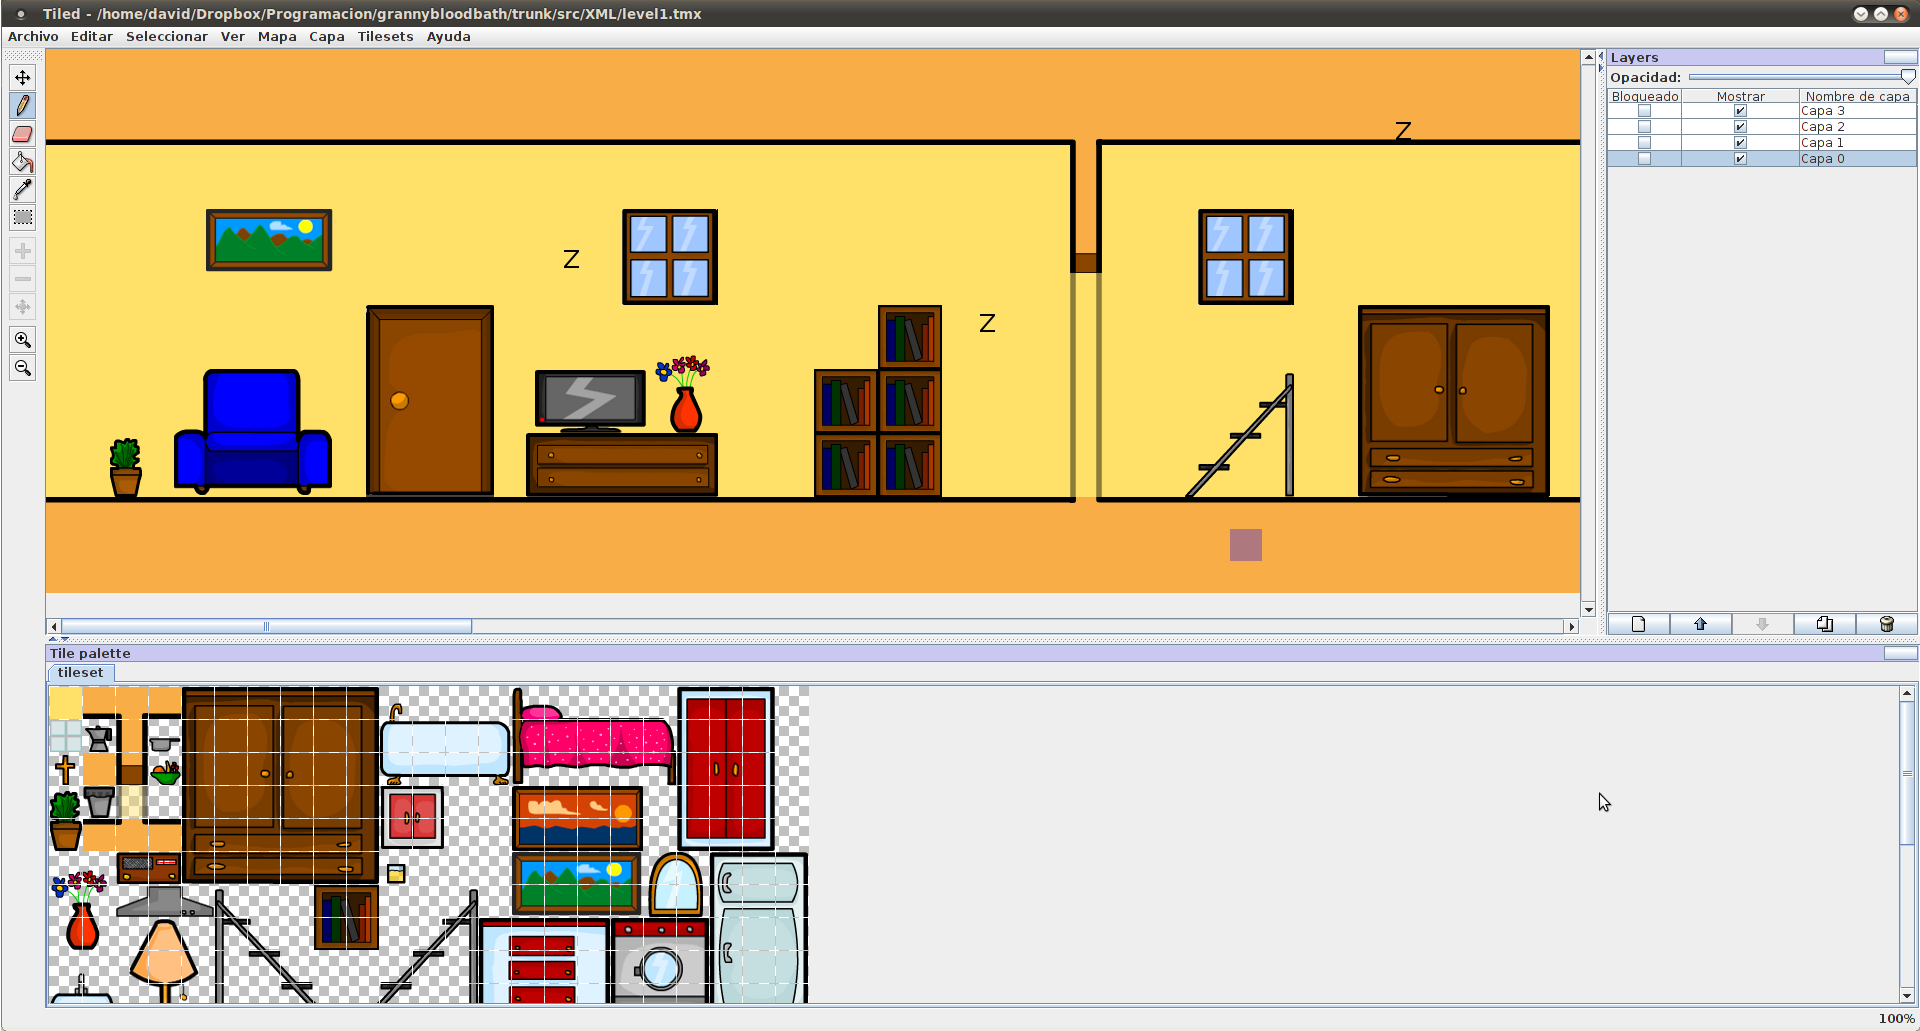
\includegraphics[scale=0.18]{tiled01.png}
\end{center}

Tiled es muy sencillo e intuitivo pero a continuación te explicamos los
elementos básicos de la interfaz para que puedas crear escenarios en un
plis plas:

\begin{itemize}
	\item \emph{Paleta de herramientas}: el panel de la izquierda es
	la barra donde se encuentran las distintas herramientas. Básicamente
	utilizarás el lápic (colocar tiles) y la goma de borrar (eliminar
	tiles).
	\item \emph{Paleta de tiles}: el panel inferior es donde se carga
	el tilset seleccionado. Un tileset es como la paleta de un pintor,
	vas poniendo cuadraditos con la herramienta de lapiz (o tiles) para 
	formar el escenario, como un puzzle. Puedes seleccionar varios
	tiles a la vez arrastrando el raton.
	\item \emph{Barra de capas}: el panel de la derecha es el de las capas
	un escenario de Granny's Bloodbath se compone de 4 capas, las cuales
	explicaremos en el siguiente apartado.	
	\item \emph{Menú}: el típico menú de cualquier aplicación. Desde allí
	podemos cargar niveles, crear nuevos niveles o guardar niveles. También
	podemos cambiar las propiedades y dimensiones del nivel actual.
\end{itemize}

\subsection{Creando escenarios con Tiled desde 0}

El siguiente tutorial explica, paso a paso, cómo hacer un nivel en Tiled para
\emph{Granny's Bloodbath} desde 0. Si quieres ahorrarte complicaciones como
los pasos 2, 3 y 5 puedes elegir un nivel vacío ya configurado en la carpeta
\emph{niveles\_vacios} dentro del directorio del juego.

\begin{enumerate}
	\item Hacemos click en Archivo $\rightarrow$ Nuevo. Nos aparece un diálogo
	y tenemos que seleccionar:
	\begin{itemize}
		\item Tipo de mapa: ortogonal
		\item Tamaño de mapa: anchura la deseada, altura 17 (si
		seleccionamos una altura de tile de 32).
		\item Tamaño de tile: dimensiones de los tiles del tileset
		que utilizaremos. Generalmente $32x32$.
	\end{itemize}
	\item Hacemos click en Tilesets $\rightarrow$ Nuevo tileset. Nos aparece
	un nuevo diálogo que rellenamos de la siguiente manera:
	\begin{itemize}
		\item Nombre del tileset: el deseado
		\item Ancho y alto de tile: como hemos dicho, normalmente
		será 32.
		\item Seleccionamos el checkbox para cargar una imagen y
		pulsamos Navegar para elegirla. Debería estar en el directorio
		multimedia de la carpeta de Granny's Bloodbath.
	\end{itemize}
	\item Creamos las 4 capas necesarias haciendo click sobre el botón
	Añadir capa del panel de capas.
	\begin{itemize}
		\item \emph{Capa 0}: fondo, paredes y objetos que ocupan
		todo el tile.
		\item \emph{Capa 1}: tiles que tienen zonas transparentes,
		se superponen sobre el fondo.
		\item \emph{Capa 2}: tiles que se visualizarán encima de los
		personajes (como si ellos estuvieran por detrás).
		\item \emph{Capa 3}: enemigos y objetos.
	\end{itemize}
	\item Trabajamos rellenando el escenario con los tiles del tileset.
	Presta atención a la capa que tienes seleccionada ya que es posible
	equivocarse. Puedes volver atrás pulsando $Ctrl+Z$.
	\item Ahora debes hacer click en Mapa $\rightarrow$ Propiedades para
	rellenar algunos datos sobre tu nivel:
	\begin{itemize}
		\item tileset\_ancho: número de tiles de ancho del tileset.
		\item tileset\_alto: número de tiles de alto del tileset.
		\item music: código de la música que debe sonar en el nivel.
		Encontrarás los códigos disponibles en el fichero
		XML/resources.xml.
		\item zombie: número de tile del personaje zombie. Normalmente
		viene indicado con una Z. Los números empiezan en 0.
		\item dog: número de tile del perro zombie. Normalmente
		viene indicado con una D. Los números empiezan en 0.
		\item fat: número de tile del zombie gordito. Normalmente
		viene indicado con una F. Los números empiezan en 0.
		\item ammo: número de tile de la munición. Normalmente
		viene indicado con una A. Los números empiezan en 0.
		\item pills: número de tile de las pastillas para la tensión. Normalmente
		viene indicado con una P. Los números empiezan en 0.
		\item teeth: número de tile de la dentadura postiza. Normalmente
		viene indicado con una T. Los números empiezan en 0.
	\end{itemize}
	\item Una vez terminado el mapa hacemos click en Archivo $\rightarrow$
	Guardar como. Elegimos la ruta y el nombre, normalmente deberíamos guardarlo
	en la carpeta XML donde esté situado Granny's Bloodbath.
	\item Para añadir nuestro nuevo nivel al guión tenemos que editar el fichero XML
	XML/plot.xml. Si nuestro nivel se llama `minivel.tmx' el fichero plot.xml
	quedaría de la siguiente manera:\\
	
	\lstinputlisting{plot.xml}
	
	Si nuestro nivel fuera la escena de un enemigo final, en lugar de `level'
	debemos introducir el atributo `boss'.
	
	\item El último paso pasa por editar el fichero del nivel y cambiar la propiedad
	\emph{source} del elemento \emph{image} dentro de \emph{tileset} de:\\
	
	\emph{../multimedia/mi-tileset.png}\\
	
	a:\\
	
	\emph{multimedia/mi-tileset.png}
\end{enumerate}


\clearpage

\section{Contacto y soporte}
Si tienes cualquier problema con \emph{Granny's Bloodbath} te pedimos, por favor que realices las siguientes acciones en el orden nombrado:

\begin{enumerate}
	\item Consultar la web por si existe alguna versión más reciente que solucione tu problema:\\
	\href{http://grannysbloodbath.wordpress.com/descargas/}{http://grannysbloodbath.wordpress.com/descargas/}
	\item Visitar la forja en caso de que haya algún mensaje, noticia o bug que anuncie el problema:\\
	\href{https://forja.rediris.es/projects/grannybloodbath/}{https://forja.rediris.es/projects/grannybloodbath/}
	\item Ponte en contacto con los desarrolladores a través del formulario habilitado a tal efecto en el blog (absténganse de tirarnos piedras, por favor):\\
	\href{http://grannysbloodbath.wordpress.com/contacto/}{http://grannysbloodbath.wordpress.com/contacto/}
\end{enumerate}

Si quieres felicitarnos, alabarnos o incluso regalarnos una pata de jamón por los buenos ratos puedes ponerte en contacto con nosotros a través del blog.


\clearpage
\section{Créditos}
\begin{itemize}
	\item \textbf{Desarrollo}:
		\begin{itemize}
			\item David Saltares Márquez
			\item Jose Marente Florín
			\item Manuel de la Calle Brihuega
		\end{itemize}		
	\item \textbf{Grafismo y animación}:
		\begin{itemize}
			\item David Saltares Márquez
			\item Jose Marente Florín
		\end{itemize}
	\item \textbf{Doblaje}:
		\begin{itemize}
			\item Ainhoa Martínez Góngora
			\item David Saltares Márquez
			\item Jose Marente Florín
		\end{itemize}
	\item \textbf{Banda sonora}:
		\begin{itemize}
			\item Fremito
			\item Ozzed
		\end{itemize}
	\item \textbf{Efectos de sonido}:
		\begin{itemize}
			\item David Saltares Márquez
			\item Jose Marente Florín
			\item Manuel de la Calle Brihuega
		\end{itemize}
\end{itemize}


\clearpage

\section{Licencia}
Este documento forma parte de \emph{Granny's Bloodbath}, publicado bajo licencia GNU Free Documentation License
Para más detalles consulte el siguiente enlace:\\

\href{http://www.gnu.org/licenses/fdl.html}{http://www.gnu.org/licenses/fdl.html}


\end{document}

